\documentclass[12pt,a4paper]{article}

\usepackage{graphicx}

\usepackage{hyperref} % this for link

\usepackage{sectsty}
\sectionfont{\fontsize{12}{15}\selectfont}

\usepackage{pdfpages}

\usepackage[left=3.175cm,right=3cm,top=3cm,bottom=3cm]{geometry}

\begin{document}


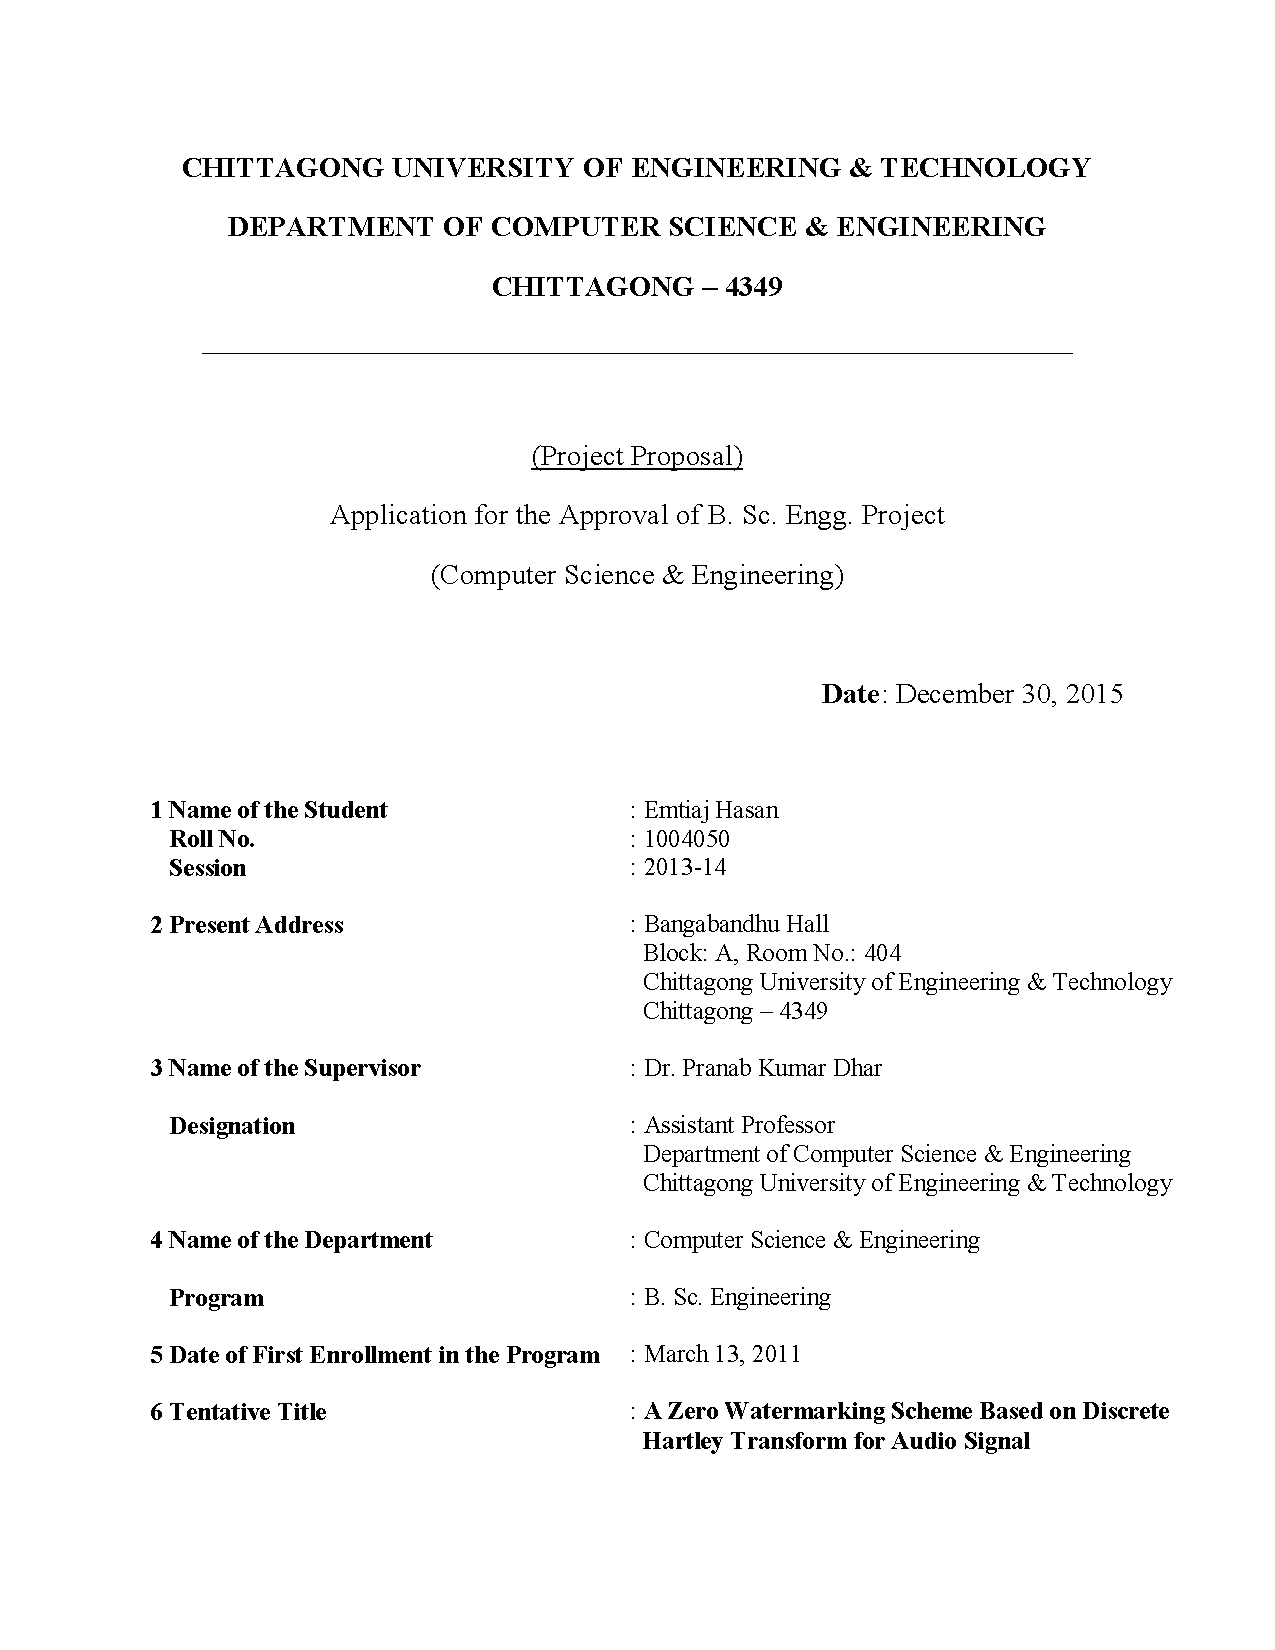
\includepdf[pages={1}]{proposalfirstpage.pdf}

\setcounter{section}{6}
\setcounter{page}{1}


\section{Introduction}


In this era of technologically advanced world, there are new opportunities for the creation and delivery of content in digital form such as images, video, audio, text. This enables easily accessible by ordinary people around the world for sharing, purchasing, distributing, or many other purposes. As a result of this, such digital products are facing serious challenges like piracy, illegal redistribution, ownership claiming, forgery, theft, etc. Digital watermarking technology is an effective solution to meet such challenges.

\bigskip

A watermark is considered to be some kind of information that is embedded into underlying data for tamper detection, localization, ownership proof, traitor tracing, etc. In visible digital watermarking, the information is visible in the picture, text or video. In invisible digital watermarking, information is added as digital data to audio, text, picture or video.

\bigskip

Digital watermarking described methods and technologies that hide information, for example, a number or text in digital media such as image, audio or video. The hiding process has to be such that the modification of the media are imperceptible. Furthermore, the watermark must be either robust or fragile, depending on the application.A watermark is called fragile if detection fails with even minor modification. It is useful in tempering detection. A watermark is called robust if detection is accurate under any modification. It is used in copyright control application.

\bigskip

Recently, many efforts have been devoted to the problem of digital audio copyright protection by plenty of research communities. This is because that multimedia data has become a widely used carrier of information and the rapid growth of Internet has made the copyright and integrity of audio information more and more important issues. To protect digital works against illegal use and tampering, digital watermarking has been proposed to accomplish copyright protection or content
integrity authentication.

\section{Background and Present State of the System}

In traditional audio watermarking techniques, either in
spatial domain, transform domain, or dual domaim \cite{wang, wqi} the embedding of watermark into the host audio inevitably introduces some audible quality degradation. Another problem is the inherent conflict between the imperceptibility and robustness.

\bigskip

Zero watermarking technique is a new approach in audio watermarking field. Here audio signal is not altered to embed watermark rather the characteristics of audio are utilized to generate a watermark. Furthermore, the
zero watermarking technology gives an effective solution to the problems of various attack such as compression, re-sampling, filtering, etc.

\bigskip

A zero watermarking scheme has been proposed to analyze the security of audio signals \cite{zws} presented a method for mapping the approximate coefficients of the wavelet transform of an audio segment into a binary matrix. A zero-watermarking algorithm, based on the Discrete Wavelet Transform (DWT), has been used to construct secrete keys \cite{dwt}. DWT and Discrete Cosine Transformation (DCT) have been combined to generate the watermarking sequences \cite{ieee, eurasip}. An audio zero-watermarking algorithm that combined DCT and Zernike moments \cite{zernik} discovered that the entropy of an audio signal on different scales yielded its statistical features. The concept of the zero-watermark based on energy was also proposed to protect audio signals \cite{energy}. However, the main weakness of the existing algorithms is poor ability of anti-attack.

\section{Objective with Specific Aims and Possible Outcomes}


\begin{itemize}

\item 
To design an algorithm to generate a watermark by utilizing the characteristics of audio.

\item
Extraction of watermark to verify the ownership of audio.

\end{itemize}


\section{Outline of Methodology}

Methodology of the proposed approach consists of two algorithms mainly:

\begin{enumerate}
\item Watermark key generation.
\item Extraction of watermarked image.
\end{enumerate}

For watermark key generation, method shown in Fig. \ref{fig:embedding} at page \pageref{fig:embedding}, Discrete Hartley Transform (DHT) is performed on audio. Then, the coefficients that have been found after performing DHT, is divided into an arbitrary number of frames. Then, binary pattern is generated, with which XOR operation is performed with a watermark, which is a binary valued image.

\begin{figure}[h!]
\centering
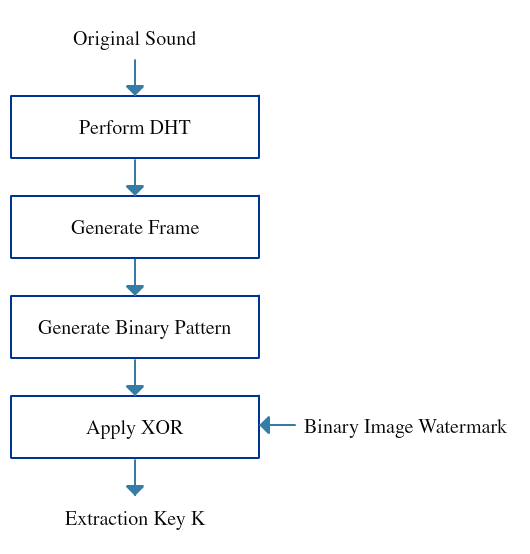
\includegraphics[scale=.7]{image/Embedding(proposal).png}
\caption{Watermark embedding process}
\label{fig:embedding}
\end{figure}

\newpage

Watermark extraction process shown in Fig. \ref{fig:extraction} at page \pageref{fig:extraction}, DHT is performed on watermarked audio. Then, the coefficients that have been found after performing DHT, is divided into an arbitrary number of frames. Then, binary pattern is generated. Then XOR operation is applied between binary pattern and the key that has been found from embedding process. That results the extraction of the watermarked image.

\begin{figure}[h!]
\centering
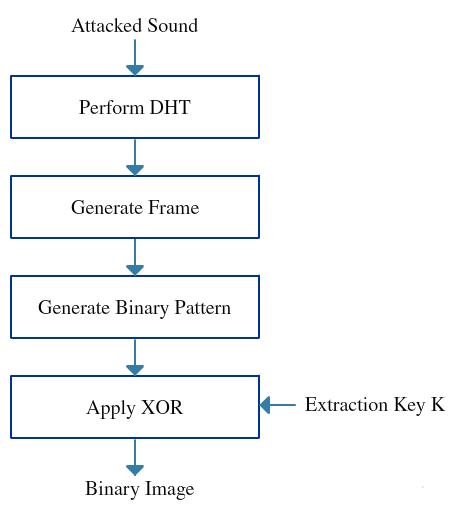
\includegraphics[scale=.7]{image/Extraction(proposal)}
\caption{Watermark extraction process}
\label{fig:extraction}
\end{figure}

\newpage

\section{Resources Required for Completing the Work}

\begin{itemize}
\item Personal Computer
\item Operating System - Windows 8
\item Processing Software - Matlab
\end{itemize}

\section{Cost Estimation}

Not applicable.

\newpage

\bibliographystyle{IEEEtran}
\bibliography{IEEEabrv,references}

\newpage


\section{CSE Undergraduate Studies (CUGS) Committee Reference}

{\hspace*{10mm}Meeting No: \hspace{20mm}
Resolution No:\hspace{25mm} Date:
}

\section{Number of Under-Graduate Student(s) Working with the Supervisor at Present}

\hspace{9mm} 09

\vspace{40mm}

\begin{flushright}
\noindent \rule{4.5cm}{0.4pt} \\
Signature of the Student

\bigskip
\bigskip
\bigskip
\bigskip

\noindent \rule{5cm}{0.4pt} \\
Signature of the Supervisor

\bigskip
\bigskip
\bigskip
\bigskip

\noindent \rule{7.4cm}{0.4pt} \\
Signature of the Head of the Department

\end{flushright}


\end{document}


